\chapter{随机变量的数值特征}
\begin{introduction}[考试重点]
    \item 重期望公式
    \item 重方差公式
    \item 切比雪夫不等式
\end{introduction}
\section{期望}

\begin{definition}[期望]
    对于实值随机向量$X : (\Omega,\mathscr{F},\P) \to (\R,\mathscr{B}_{\R})$和(可测)函数$g : \Rn \to \R$,若
    \[ \E[g(X)] = \int_{\R} g(x) \mathrm{d} F_X(x) \]
    存在,则称其为$g(X)$的\textbf{期望}(expectation)。
\end{definition}

\begin{remark}
    当$F_X(x)$在$x_0$初连续可导时,$\mathrm{d} F_X(x_0)=f_X(x_0)\d x$;当$x_0$为其间断点时时,$\d F_X(x_0)=p_{X}(x_0)\delta(x_0)\d x$。
\end{remark}

%期望算子$\E$是一个线性泛函, 仅适用于\underline{可积}的随机变量.

\begin{proposition}[期望的线性性质]
    由积分的线性性质可得:均值为随机变量的线性映射,即
    \[ \E(a+\sum_{i=1}^n b_i g(X_i))=a+\sum_{i=1}^n b_i \E(g(X_i)) \]
\end{proposition}

\begin{theorem}[Markov不等式]
    设$g(x)$为随机变量$X$取值的集合上的非负不减函数,且$E(g(X))$存在,则
    \[ P(X>\e) \leq \frac{E(g(X))}{g(\e)} ,\quad \forall \e > 0\]
\end{theorem}
\begin{proof}
    \begin{align*}
        P(X>\e) & =\int_{\e}^{+\infty}p(x) \d x \leq \int_{\e}^{+\infty}\frac{g(X)}{g(\e)}p(x) \d x \\
                & \leq \int_{-\infty}^{+\infty}\frac{g(X)}{g(\e)}p(x) \d x = \frac{E(g(X))}{g(\e)}
    \end{align*}
\end{proof}

\begin{corollary}
    若$g(X) \ge 0$,则
    \[ \E[g(X)] = 0 \Leftrightarrow  \P\{g(X)=0\} = 1 \Leftrightarrow g(X) \overset{\as}{=} 0 \]
\end{corollary}

\begin{proposition}[独立变量的期望]
    若$X,Y$\underline{独立},则
    \begin{gather*}
        \E(XY)=\E(X)\E(Y) \\
        \E(g(X)h(Y))=\E(g(X))\E(h(Y))
    \end{gather*}
\end{proposition}

\begin{remark}
    由于$\E(X/Y)= \E(X)\E(\frac1{Y})$, 而$\E(\frac1{Y}) \neq \frac1{\E(Y)}$, 所以$\E(X/Y)\neq \E(X)/\E(Y)$
\end{remark}

\begin{theorem}[Jensen不等式]
    若$g$为\underline{下凸(convex)函数},则$g[\E(X)] \le \E[g(X)]$;若$g$为\underline{上凸(concave)函数},则$\E[g(X)] \le  g[\E(X)]$。
\end{theorem}
\begin{proof}
    若$f$为凸函数,则
    \[ f(t_1x_1+t_2x_2) \le t_1f(x_1)+t_2f(x_2) ,\quad \forall t_1,t_2 \ge 0 ,\ t_1+t_2=1 \]
    由归纳可得:
    \[ f(t_1x_1+ \cdots +t_nx_n) \le t_1f(x_1)+ \cdots +t_nf(x_n) ,\quad \forall t_1,\cdots ,t_n \ge 0 ,\ t_1+ \cdots +t_n=1 \]
    拓展到连续函数:
    \[ f(\int_{X}g(x)x \d x) \le \int_{X}g(x)f(x) \d x ,\quad \forall g(x) \ge 0 ,\ \int_{X}g(x) \d x=1 \]
\end{proof}

\begin{figure}[h]
    \centering
    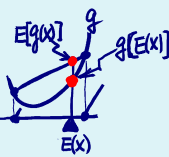
\includegraphics{image/trans_mean.png}
\end{figure}

\section{均值与方差}

\begin{definition}
    \begin{enumerate}
        \item 当$g(x)=x$时,$\E[g(x)]=\E[X]$称作$X$的\textbf{均值}(mean),记为$\mu_{X}$
        \item 当$g(x)=(x-\mu_{X})^{2}$时,$\E[g(x)]=\E[(X-\E[X])^{2}]$称作$X$的\textbf{方差}(variance),记为$\sigma^2_{X}$。其平方根称作$X$的\textbf{标准差}(standard deviation),记为$\sigma_{X}$
        \item 当$g(x,y)=(x-\mu_{X})(y-\mu_{Y})$时,$\E[g(X,Y)]=\E[(X-\E[X])(Y-\E[Y])]$称作$X$与$Y$的\textbf{协方差}(covariance),记为$\Cov(X,Y)$或$\sigma_{XY}$
    \end{enumerate}
\end{definition}

\subsection{均值}

随机变量的均值可看作其加权平均,权重为其pdf或pmf,结果为其函数图像上的形心。从大数定律(第\ref{sec:large_number}节)的角度看,也可解释为其长期均值。

\begin{example}
    在一个人数为$N$的人群中普查某种疾病,为此要抽验$N$个人的血。如果将每个人的血分别检验,则共需检验$N$次。为了能减少工作量,一位统计学家提出一种方法:按$k$个人一组进行分组,把同组$k$个人的血样混合后检验,如果这混合血样呈阴性反应,就说明此$k$个人的血都呈阴性反应,此$k$个人都无此疾病,因而这$k$个人只要检验1次就够了,相当于每个人检验$1/k$次,检验的工作量明显减少了。如果这混合血样呈阳性反应,就说明此$k$个人中至少有一人的血呈阳性反应,则再对此$k$个人的血样分别进行检验,因而这$k$个人的血要检验$1+k$次,相当于每个人检验$1+1/k$次,这时增加了检验次数。假设该疾病的发病率为$p$,且得此疾病相互独立。试问此种方法能否减少平均检验次数?
\end{example}
\begin{solution}
    令$X$为该人群中每个人需要的验血次数,则$X$的分布列为
    \begin{table}[htbp]
        \centering
        \begin{tabular}{c|cc}
            $x$ & $1 / k$   & $1+1 / k$   \\\midrule
            $P$ & $(1-p)^k$ & $1-(1-p)^k$ \\
        \end{tabular}
    \end{table}
    所以每人平均验血次数为
    \[ E(X)=\frac1{k}(1-p)^k+(1+\frac1{k})[1-(1-p)^k]=1-(1-p)^k+\frac1{k} \]
    由此可知,只要选择$k$使
    \[ 1-(1-p)^k+\frac1{k}<1,\ \text{即} ,\ (1-p)^k>\frac1{k} \]
    就可减少验血次数,而且还可适当选择$k$使其达到最小。
\end{solution}

\begin{example}[凑一法求解二项分布的均值]\label{ex:binom_dist_mean}
    求解二项分布(定义\ref{def:binom_dist})的均值时,可通过将其凑成概率质量函数之和(为1)的形式,称此为\textbf{凑一法}(sum to one, STO):
    \begin{align*}
        E(X) & =\sum_{i=1}^n x \binom{n}{x} p^x (1-p)^{n-x}                 \\
             & = np \sum_{i=1}^n \binom{n-1}{x-1} p^{x-1} (1-p)^{n-1-(x-1)} \\
             & =np
    \end{align*}
\end{example}

\begin{example}[微分法求解几何分布均值]\label{ex:geometric_dist_mean}
    \begin{align*}
        E(X) & =p\sum_{k=1}^{\infty}k q^{k-1}=p\frac{d}{d q}\sum_{k=1}^{\infty} q^{k} \\
             & =p\frac{d}{d q} \frac{q}{1-q} =\frac{p}{(1-p)^{2}}                     \\
             & =\frac{1}{p}                                                           \\
    \end{align*}
\end{example}

\begin{proposition}\label{prop:mean_of_non-negative_discrete_varible}
    设$X$为仅取非负整数的离散随机变量,若其数学期望存在,则
    \[ E(X) = \sum_{k=1}^{+\infty}P(X \ge k) \]
\end{proposition}

\subsection{方差}

方差为随机变量距其均值的均方偏差,刻画了$X$的变动程度。随机变量的均值与标准差的单位和其本身的相同,方差的为其平方。如果随机变量$X$的数学期望存在, 其方差不一定存在;而当$X$的方差存在时,则$E(X)$必定存在,其原因在于$|x| \le x^2+1$($0 \le x^2-2|x|+1$)总是成立的(若$E(X^2)$收敛,则$E(|X|)$收敛)。

\begin{proposition}
    \[ \operatorname{Var}(X)=\E[(X-\mu_X)^2]=E(X^2)-\mu_X \]
\end{proposition}

\begin{example}[凑一法求解二项分布的方差]\label{ex:binom_dist_var}
    \begin{align*}
        E(X(X-1))             & =\sum_{i=1}^n x(x-1) \binom{n}{x} p^x (1-p)^{n-x}                   \\
                              & = n(n-1)p^2 \sum_{i=1}^n \binom{n-2}{x-2} p^{x-2} (1-p)^{n-1-(x-1)} \\
                              & =n(n-1)p^2                                                          \\
        \operatorname{Var}(X) & =  E(X(X-1)) + E(X) - (E(X))^2                                      \\
                              & = n(n-1)p^2 + np -n^2 p^2                                           \\
                              & =np(1-p)
    \end{align*}
\end{example}

\begin{example}[微分法求解几何分布方差]\label{ex:geometric_dist_var}
    \begin{align*}
        E(X(X-1))             & =p\sum_{k=1}^{\infty}k(k-1) q^{k-1}=p\frac{d}{d q}\sum_{k=1}^{\infty} q^{k} \\
                              & =p\frac{d^2}{d q^2} \frac{q}{1-q} =\frac{2p}{(1-q)^{3}}                     \\
                              & =\frac{2}{p^2}                                                              \\
        \operatorname{Var}(X) & =  E(X(X-1)) + E(X) - (E(X))^2                                              \\
                              & = \frac{2}{p^2} + \frac{1}{p} -\frac{1}{p^2} p^2                            \\
                              & = \frac{1-p}{p^2}
    \end{align*}
\end{example}

\begin{proposition}
    \[ \operatorname{Var}(a+bX)=b^2\operatorname{Var}(X) \]
\end{proposition}

\begin{proposition}
    \[ \operatorname{Var}(a+\sum_{i=1}^n b_i X_i)=\sum_{i=1}^n b_i^2 \operatorname{Var}(X_i)+\mathbf{b}^{\mathrm{T}} \Sigma \mathbf{b}\]
    其中$\Sigma$为协方差矩阵,$\Sigma_{i,j}=\operatorname{Cov}(X_i,X_j)$
\end{proposition}

\begin{corollary}
    若$X_1,\cdots ,X_n$相互独立, 则:
    \[ \operatorname{Var}(\sum_{i=1}^n X_i)=\sum_{i=1}^n\operatorname{Var}( X_i) \]
\end{corollary}

\begin{theorem}[Chebyshev不等式]
    设随机变量$X$的均值与方差分别为:$\mu, \sigma^2$, 则:
    \[ \P(\left| X-\mu \right| >t)\le \frac{\sigma^{2}}{t^{2}} \]
\end{theorem}

\begin{proof}
    设$F(x)$为$X$的分布函数, 令$R=\left\{ x:|x-\mu|>t \right\}$
    \begin{align*}
        \P(|x-\mu|>t) & = \int_R 1 \cdot  \d F(x) \le \int_R \frac{(x-\mu)^2}{t^{2}}\d F(x)                   \\
                      & \le \int_{-\infty}^{\infty}\frac{(x-\mu)^2}{t^{2}}\d F(x)  = \frac{\sigma^{2}}{t^{2}}
    \end{align*}
\end{proof}

\begin{remark}
    若令$t=k\sigma$, 则$\P(| X-\mu | >k\sigma)\le \frac1{k^{2}}$, 即标准差可代表随机变量偏离均值的概率单位距离.
\end{remark}

\begin{corollary}
    \[ \operatorname{Var}(X)=0 \Leftrightarrow P(X=\mu)=1 \]
\end{corollary}

预处理随机变量有两个常用变换:
\begin{itemize}
    \item \textbf{中心化}(centralization)$X \mapsto X-\E{X}$;
    \item \textbf{标准化}(standardization)$X \mapsto \dfrac{X-\E{X}}{\sqrt{\Var(X)}}$.
\end{itemize}

\subsection{协方差}

协方差代表了$X$与$Y$之间的联合变化倾向, 或者说他们间的相关程度, 但其间\underline{未必有}因果关系.

\begin{theorem}
    \[ \operatorname{Cov} (X,Y)=\E[(X-\mu_X)(Y-\mu_Y)]=\E(XY)-\mu_Y \mu_Y \]
\end{theorem}

\begin{theorem}
    \[ \operatorname{Cov}(a+\sum_{i=1}^n b_i X_i,c+\sum_{j=1}^m d_j Y_j) = \sum_{i=1}^n\sum_{j=1}^m b_i d_j \operatorname{Cov}(X_i,Y_i) = \mathbf{b}^{\mathrm{T}}\Sigma \mathbf{d}\]
\end{theorem}

\begin{theorem}
    独立是不相关的\textbf{充分条件}, 但不是必要条件
\end{theorem}

\begin{theorem}
    $-1\le \rho_{XY} \le 1$, 当且仅当$X$与$Y$间为线性关系时取等号
\end{theorem}

\begin{proof}
    %TODO
\end{proof}

\begin{theorem}
    平移与缩放随机变量都不影响其协方差, 即:
    \[ \left| \operatorname{Cov}(a+ b X,c +d Y) \right| = \left| Cor(X,Y) \right|  \]
\end{theorem}

\section{条件期望}

\begin{definition}
    若$h(Y)$在给定$X=x$下的条件分布(定义\ref{def:cond_dist})的数学期望存在,则定义其为\textbf{条件期望}如下:
    \[ E(h(Y)|X=x) =\begin{cases}
            \sum_{y} h(y) p_{Y|X}(y|x),                    & \text{离散情况} \\
            \int_{-\infty}^{+\infty} h(y) f_{Y|X}(y|x) d y & \text{连续情况}
        \end{cases}\]
\end{definition}

\begin{remark}
    条件期望$\E_{Y|X}(Y|x)$是关于给定变量$x$的函数,不随对应变量$Y$本身变动,但其单位与对应变量$Y$相同,可看作一条在$(X,Y)$平面的曲线。
\end{remark}

\begin{theorem}
    若随机变量$X,Y$独立,则:
    \[ \E_{Y|x}(Y|x)=\E_{Y}(Y) \]
\end{theorem}

\begin{proof}
    由\ref{thm:indep_cmf}可知,若随机变量$X,Y$独立,则
    \begin{align*}
        p_{Y|X}(y|x) & =p_{Y}(y) \\
        f_{Y|X}(y|x) & =f_{Y}(y)
    \end{align*}
    所以$\E_{Y|x}(Y|x)=\E_{Y}(Y)$
\end{proof}

由直观感受亦可知:若$X,Y$独立,则$X$不通过任何与$Y$相关的信息,其条件期望亦当与原期望相同。

\begin{note}
    令$g(x)=\E(h(Y)|X=x)$,则$g(X)$是随机变量$X$的变换,也是随机变量,记为$\E(h(Y)|X)$
\end{note}

\begin{theorem}[重期望公式]
    \[ \E_X[\E_{Y|X}(h(Y)|X)] = \E_{Y}[h(Y)] \]
\end{theorem}

\begin{proof}
    %TODO
\end{proof}

\begin{theorem}
    联合期望公式:
    \[ E_{X,Y}=E_X E_{Y|X} = E_Y E_{X|Y} \]
    泛化情况:
    \[ E_{X,Y}[h(X,Y)]=E_X E_{Y|X}[h(X,Y)|X] = E_Y E_{X|Y}[h(X,Y)|Y] \]
\end{theorem}

\begin{theorem}[重方差公式]\label{thm:var_dec}
    随机变量$Y$的方差可作如下分解:
    \[ \operatorname{Var}_Y(Y)=\operatorname{Var}_X[E_{Y|X}(Y|X)] + E_X[\operatorname{Var}_{Y|X}(Y|X)] \]
\end{theorem}

\begin{figure*}
    \centering
    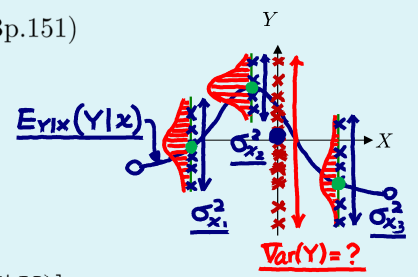
\includegraphics{image/var_dec.png}
\end{figure*}

\begin{corollary}
    \[ \operatorname{Var}_Y(Y) \ge E_X[\operatorname{Var}_{Y|X}(Y|X)] \]
    当且仅当$E_{Y|X}(Y|X)=E_Y(Y)$时取等号
\end{corollary}

\begin{figure*}
    \centering
    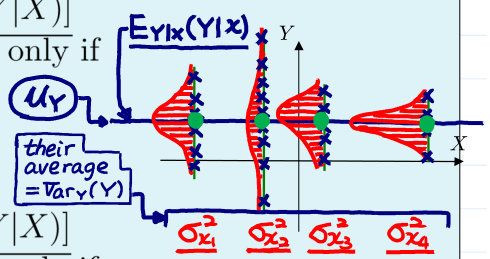
\includegraphics{image/var_dec2.png}
\end{figure*}

\begin{corollary}
    \[ \operatorname{Var}_Y(Y) \ge \operatorname{Var}_X[E_{Y|X}(Y|X)] \]
    当且仅当$\operatorname{Var}_{Y|X}(Y|X)=0$,即$\E_{Y|X}(Y|X)=Y$时取等号
\end{corollary}

\begin{figure*}
    \centering
    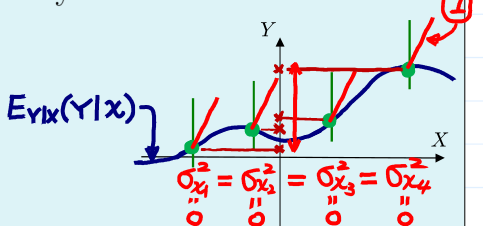
\includegraphics{image/var_dec3.png}
\end{figure*}

\section{矩母函数与特征函数}

\subsection{矩}

\begin{definition}
    对于随机变量$X$, 定义其$k$阶\textbf{矩}(moment)为$E(X^k)$, 记为$\mu_k$; 定义其$k$阶\textbf{中心矩}(central moment)为$E((X-\mu_X)^k)$, 记为$\upsilon_k$;
\end{definition}

易知矩与中心矩间存在以下关系:
\begin{align*}
    \upsilon_k & =\sum_{i=0}^k \binom{k}{i} \mu_i (-\mu_X)^{n-i}     \\
    \mu_k      & =\sum_{i=0}^k \binom{k}{i} \upsilon_i (\mu_X)^{n-i}
\end{align*}

特别的有:
\begin{align*}
    E(X)                  & =\mu_1                                                         \\
    \operatorname{Var}(X) & =\upsilon_2=\mu_1^2-2\mu_1 \cdot \mu_1 + \mu_2 = \mu_2-\mu_1^2
\end{align*}

\subsection{矩母函数}

\begin{definition}
    对于随机变量$X$, 若下式期望存在:
    \[ M_X(t) = \E(e^{tX}) \]
    则称其为\textbf{矩母函数}(moment generating function, mgf)。
\end{definition}

\begin{remark}
    此表达式等价于对概率质量函数或密度函数作Laplace变换, 当$t$取某些特定值时, 可能不存在. (若$t=0$则永远存在)
\end{remark}

\begin{theorem}
    若当$t$属于一个包含零点的开区间时, 矩母函数一直存在, 则其唯一对应一个概率分布.
\end{theorem}

\begin{theorem}
    若当$t$属于一个包含零点的开区间时, 矩母函数一直存在, 则:
    \[ M_X^{(k)}(0) = E(X^k) \]
\end{theorem}

\begin{remark}
    借此可方便地计算各阶矩, 故称为矩母函数. 反过来, 若已知各阶矩, 通过Tayler展开$M_X(t)=\sum_{k=0}^{\infty}\frac{M_X^{(k)}(0)}{k!}t^k$可还原矩母函数, 进而得出概率分布.
\end{remark}

\begin{proposition}
    若$a,b$为常数, 则
    \[ M_{a+b X}(t) = e^{a t}M_X(b t) \]
\end{proposition}

\begin{theorem}\label{thm:mgf_sum}
    若$X,Y$独立,则
    \[ M_{X+Y}(t) = M_X(t) M_Y(t) \]

    泛化情况: 若$X_1,\cdots, X_n$相互独立,则
    \[ M_{X_1+\cdots+ X_n} = \prod_{i=1}^n M_{X_i}(t)\]
\end{theorem}

\subsection{联合特征函数}

\begin{definition}
    对于随机变量$X_1,\cdots, X_n$, 若下式期望存在:
    \[ M_{X_1\cdots X_n}(t_1,\cdots ,t_n) = \E(e^{t_1 X_1+\cdots + t_n X_n}) \]
    则称其为\textbf{联合矩母函数}(joint moment generating function, joint mgf)。
\end{definition}

\begin{remark}
    此处为\underline{多元}函数
\end{remark}

\begin{proposition}
    \[ M_{X_i}(t_i) = M_{X_1\cdots X_n}(0,\cdots ,t_i,\cdots ,0) \]
\end{proposition}

\begin{theorem}
    当且仅当:
    \[ M_{X_1\cdots X_n}(t_1,\cdots ,t_n) = \prod_{i=1}^n M_{X_i}(t_i) \]
    时,$X_1,\cdots, X_n$相互独立
\end{theorem}

\begin{remark}
    与\underline{累计函数、密度函数、质量函数}的情况类似,变量相互独立等价于联合函数可拆分为边缘函数的乘积
\end{remark}

\begin{theorem}
    \[ \frac{\partial^{r_1+\cdots +r_n} }{\partial t_1^{r_1} \cdots  \partial t_n^{r_n}} M_{X_1\cdots X_n}(t_1,\cdots ,t_n) = E(X_1^{r_1} \cdots X_n^{r_n}) \]
\end{theorem}

\subsection{特征函数}

由于有时矩母函数可能不存在,为避免此缺陷,构造出与之特性类似的特征函数。

\begin{definition}
    对于随机变量$X$, 定义其\textbf{特征函数}(characat function, chf)为:
    \[ \phi_X(t) = \E(e^{itX}) = \E(\cos (tX)) + i\E(\sin (tX))\]

    对于随机变量$X_1,\cdots, X_n$, 定义其\textbf{联合特征函数}(joint characat function, joint chf)为:
    \[ \phi_{X_1\cdots X_n}(t_1,\cdots ,t_n) = \E(e^{i (t_1 X_1+\cdots + t_n X_n)}) \]
\end{definition}

\begin{remark}
    此表达式等价于对概率质量函数或密度函数作Fourier变换
\end{remark}

\begin{proposition}
    随机变量的特征函数总是存在
\end{proposition}

\begin{proposition}
    若矩母函数存在,则其与特征函数之间满足关系:
    \[ \phi_X(t) = M_X(it) \]
\end{proposition}

\begin{theorem}
    特征函数可通过以下逆变换得到分布:
    \begin{description}
        \item[离散]$p_{X}(x)=\lim _{T \rightarrow \infty} \int_{-T}^{T} e^{-i t x} \phi_{X}(t) d t$
        \item[连续]$f_X(x)=\frac1{2 \pi} \int_{-\infty}^{\infty} e^{-i t x} \phi_{X}(t) d t$
    \end{description}
\end{theorem}

\section{估计与预测}

\subsection{delta法}

\subsection{预测}

\section{熵与信息}

\subsection{费尔希信息量}



\section{其他特征}

\subsection{相关系数}

\begin{definition}
    定义$X$与$Y$的\textbf{相关系数}(correlation coefficient)为:$\sigma_{XY}/(\sigma_{X}\sigma_{Y})$, 记为$\Cor(X,Y)$或$\rho_{XY}$. 若$\rho_{XY}=0$, 则称$X$与$Y$不相关
\end{definition}

\begin{problemset}[错题记录]
    \item (茆2.2.7)对一批产品进行检查,如查到第$a$件全为合格品,就认为这批产品合格;若在前$a$件中发现不合格品即停止检查,且认为这批产品不合格。设产品的数量很大,可认为每次查到不合格品的概率都是$p$。问每批产品平均要查多少件?
    \item (茆2.2.17)设随机变量$X$的概率密度函数为
    \[ p(x)=\begin{cases}
            \frac{1}{2} \cos \frac{x}{2}, & 0 \leq x \leq \pi; \\
            0,                            & \text{其他}.
        \end{cases} \]
    对$X$独立重复观察4次,$Y$表示观察值大于$\pi/3$的次数,求$Y^2$的数学期望。
    \item (茆2.2.20)设连续随机变量$X$的分布函数为$F(x)$,且数学期望存在,证明
    \[ E(X) = \int_{0}^{+\infty}[1-F(x)] \dd  x-\int_{-\infty}^{0} F(x) \dd  x \]
    \item (茆2.2.21)设$X$是非负连续随机变量,若$E(X^n)$存在,证明:\begin{enumerate}
        \item $E(X)=\int_0^{\infty}P(X>x) \mathrm{d}x$
        \item $E(X^n)=\int_0^{\infty}n x^{n-1}P(X>x) \mathrm{d}x$
    \end{enumerate}
    \item (茆2.2.22)甲、乙两人进行象棋比赛,每局甲胜的概率为$p$,乙胜的概率为$q=1-p$。比赛进行到有一人连胜两局为止,求平均比赛局数。
    \item 设随机变量$X$的分布函数为
    \[ F(x)=\begin{cases}
            0,                                  & x<-1         \\
            \frac{1}{2}+\frac{1}{\pi}\arcsin x, & -1\le x\le 1 \\
            1,                                  & x\ge 1
        \end{cases} \]
    试求$E(X)$。
\end{problemset}
